% !TEX root = ./PS-Tests_Resolutions.2022.2.tex
\providecommand\mainfilename{"./PS-Tests_Resolutions.tex"}
\providecommand \subfilename{}
\renewcommand   \subfilename{"./PS-Tests_Resolutions.2022.2.tex"}
\documentclass[\mainfilename]{subfiles}

% \tikzset{external/force remake=true} % - remake all

\begin{document}

\graphicspath{{\subfix{./figures/PS-Tests_Resolutions.2022.2}}}
% \tikzsetexternalprefix{./figures/PS-Tests_Resolutions.2022.2/graphics/}

\mymakesubfile{2}
[PS]
{Teste 2022.2 Resolução} % Subfile Title
{Teste 2022.2 Resolução} % Part Title

\begin{questionBox}1{ % MARK: Q1
    Extrai-se ácido acético de uma solução aquosa com 60\% p/p em ácido usando para o efeito clorofórmio puro, de forma a obter um refinado final com uma concentração de ácido de 5\% p/p. Para tal, usam-se dois andares de equilíbrio, com adição de solvente fresco em cada andar, para processar \qty*{1000}{\kilo\gram/\hour} de solução aquosa. No primeiro andar de equilíbrio usa-se uma proporção entre solvente fresco e alimentação aquosa de 1:1. Calcule:
} % Q1
\end{questionBox}

\begin{questionBox}2{ % MARK: Q1.1
    as composições e caudais mássicos das correntes de saída em cada andar.
} % Q1.1
\end{questionBox}

\begin{questionBox}2{ % MARK: Q1.2
    a quantidade mínima de solvente que poderia usar no primeiro andar. Justifique a resposta.
} % Q1.2
\end{questionBox}

\begin{questionBox}2{ % MARK: Q1.3
    a percentagem total de extracção de ácido acético da solução aquosa original.
} % Q1.3
\end{questionBox}

\begin{questionBox}2{ % MARK: Q1.4
    Em que situações pensa que a extracção com solventes líquidos possa ser mais vantajosa que a destilação como processo de separação?
} % Q1.4
\end{questionBox}

\begin{questionBox}1{ % MARK: Q2
    Pretende-se arrefecer água de 45ºC a 25ºC numa torre utilizando ar em contracorrente. O caudal de água é de \qty*{1500}{\kilo\gram/\metre^2.\hour} e o caudal de ar que entra a 25ºC e com uma temperatura de termómetro húmido 21ºC é de \qty*{1250}{\kilo\gram/\metre^2.\hour}.
} % Q2
    \paragraph*{Dados:}
    \begin{itemize}
        \begin{multicols}{2}
            \item \(K_{H}\,a=\qty*{0.5}{\kilo\gram/\metre^3.\second}\)
            \item \(C_{p,agua}=\qty*{4.18}{\joule/\gram.\celsius}\)
        \end{multicols}
    \end{itemize}
    \begin{BM}
        Z
        =\frac{V'}{K_H\,a\,S}
        \int_{E_{G,1}}^{E_{G,2}}{
            \frac{\odif{E_G}}{
                E^*_G-E_G
            }
        }
        ;\qquad
        \frac{E_{G,2}-E_{G,1}}
        {T_{L_2}-T_{L_1}}
        = \left[
            \frac{\bar{L}\,c_{p,L}}{V'}
        \right]
    \end{BM}

    \begin{questionBox}2{ % MARK: Q2.1
        Determine a humidade absoluta e relativa do ar à entrada da coluna e as entalpias do ar à entrada e à saída da coluna.
    } % Q2.1
    \end{questionBox}

    \begin{questionBox}2{ % MARK: Q2.2
        Calcule \((E^*_G-E_G)^{-1}\) para a base e o topo da coluna. Comente.
    } % Q2.2
    \end{questionBox}

    \begin{questionBox}2{ % MARK: Q2.3
        Se a coluna tiver \qty*{3}{\metre} de altura, qual o número de unidades de transferência necessárias neste processo?
    } % Q2.3
    \end{questionBox}

\end{questionBox}

\begin{questionBox}12{ % MARK: Q3.1
    Caracterize o processo de secagem considerando o seu modo de operação, o método de fornecimento de calor necessário e a natureza do material sólido.
} % Q3.1
\end{questionBox}

\begin{questionBox}2{ % MARK: Q3.2
    A indústria PAPELIS SA. usa um secador de tabuleiros com dois conjuntos de tabuleiros. Na operação do secador, ar saturado a 22ºC é previamente aquecido a 75ºC, e em seguida feito passar pelo primeiro conjunto de tabuleiros. À saída desse 1º estágio, o ar sai com 60\% de saturação, sendo depois de novo aquecido a 75ºC antes de entrar no segundo conjunto de tabuleiros. À saída deste 2º estágio, o ar tem de novo 60\% de saturação. Admitindo que o processo de secagem decorre de forma adiabática calcule a temperatura final do sólido em cada conjunto de tabuleiros.
} % Q3.2
\end{questionBox}

\begin{questionBox}2{ % MARK: Q3.3
    Calcule a quantidade total de água retirada ao sólido por \unit{\kilo\gram} de ar seco.
} % Q3.3
\end{questionBox}

\begin{sectionBox}*b{} % MARK: S
    
    \begin{center}
        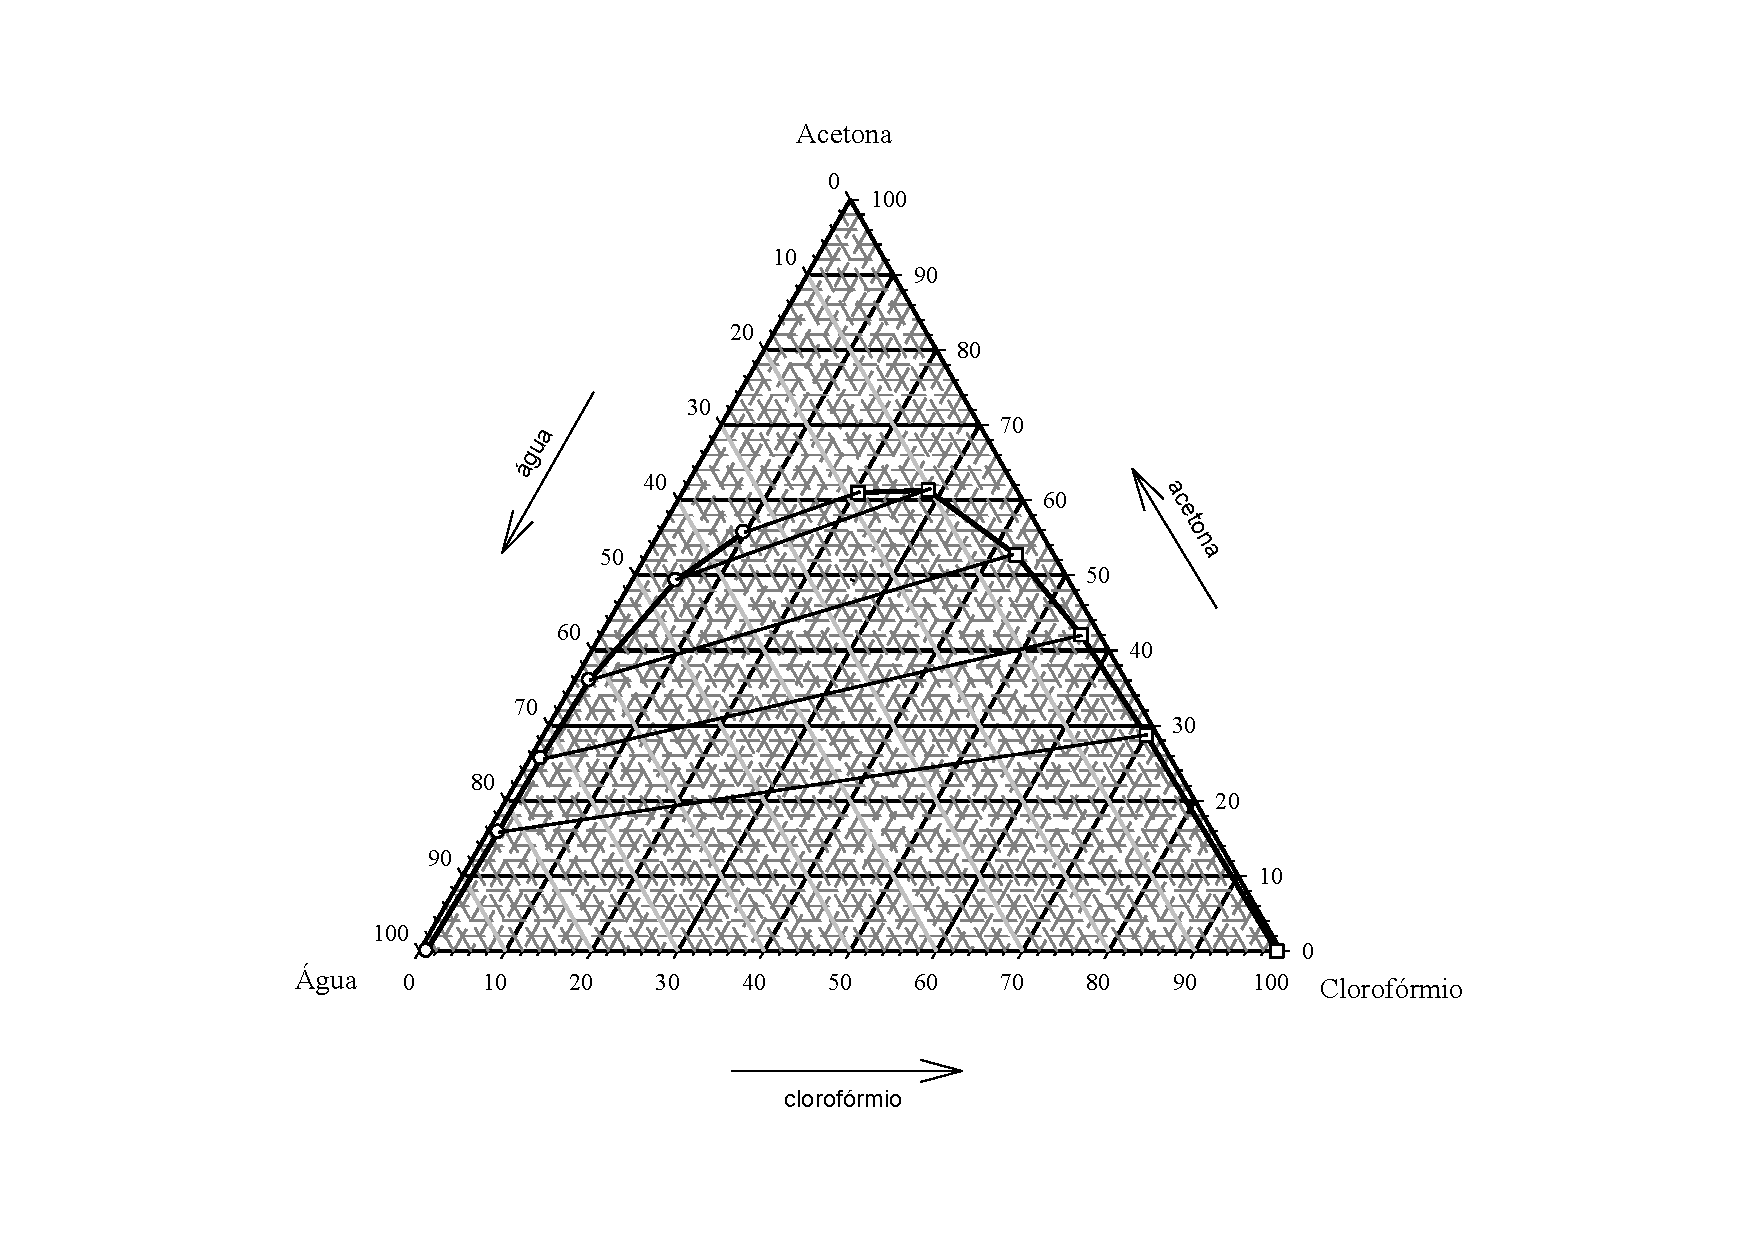
\includegraphics[width=1\textwidth]{extractedPages-page2.pdf}
    \end{center}
    
\end{sectionBox}
\begin{sectionBox}*b{} % MARK: S
    
    \begin{center}
        \includegraphics[width=1\textwidth]{-003-000.png}
    \end{center}
    
\end{sectionBox}
\begin{sectionBox}*b{} % MARK: S
    
    \begin{center}
        \includegraphics[width=1\textwidth]{-004-001.png}
    \end{center}
    
\end{sectionBox}
\begin{sectionBox}*b{} % MARK: S
    
    \begin{center}
        \includegraphics[width=1\textwidth]{-005-002.png}
    \end{center}
    
\end{sectionBox}

\end{document}